\section{Workflows Desenvolvidos}
\subsection{Acidente em Braga no ano de 2019}
    \subsubsection{Principais nodos}
        \begin{figure}[H]
            \centering
            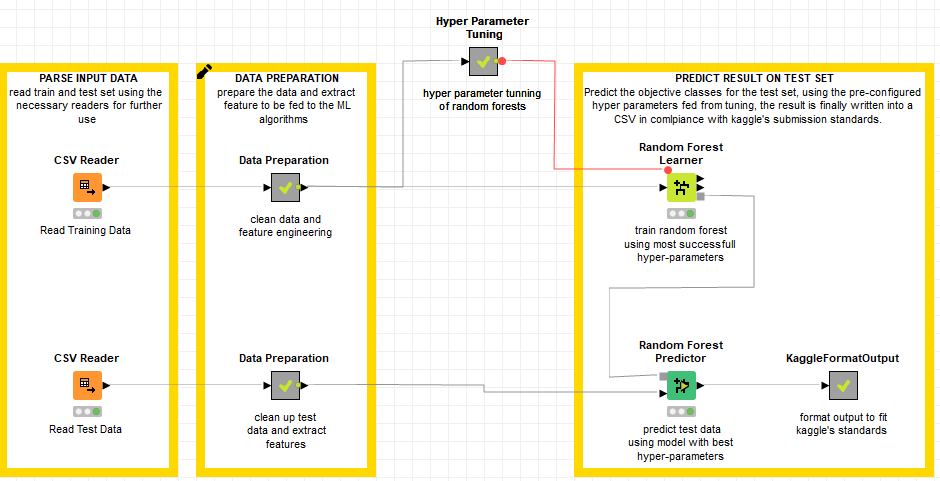
\includegraphics[scale=0.35
            ]{Figures/wf_braga.png}
            \caption{Visão geral do workflow gerado para trabalhar o \textit{dataset}.}
            \label{fig:"um"}
        \end{figure} 
        
    \begin{enumerate}
        \item \textbf{Parse Input Data} \\
            Neste ponto foram carregados para o Knime dois ficheiros, ambos com os mesmos campos de informação, relativos ao número de incidentes rodoviários em Braga. Um dos ficheiros possui dados para usar no treino do modelo, enquanto o outro possui dados para testarmos o modelo.
            
        \item \textbf{Data Preparation} \\
            Relativamente à preparação dos dados apresentamos na figura abaixo o conteúdo do metanodo desenvolvido para esse efeito.
            \begin{figure}[H]
                \centering
                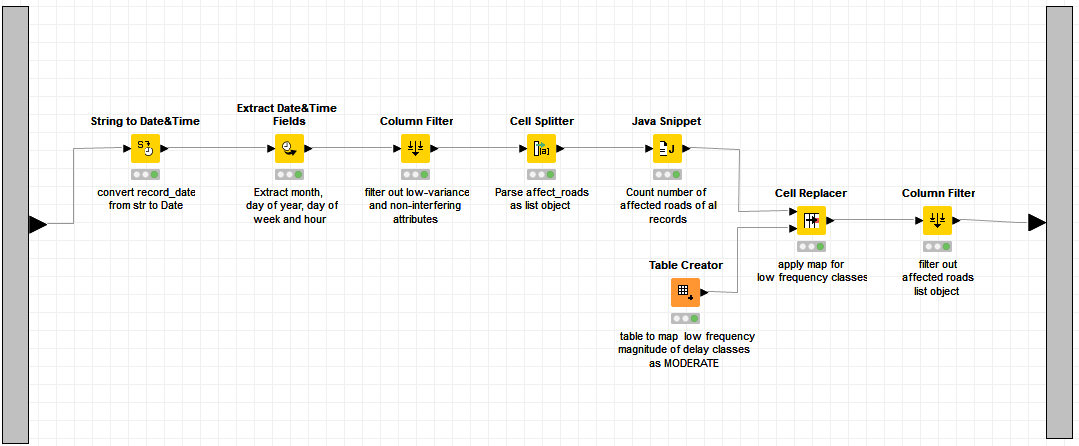
\includegraphics[scale=0.3
                ]{Figures/wf_braga_dataPrep.png}
                \caption{Visão geral do workflow gerado para trabalhar o dataset.}
                \label{fig:"um"}
            \end{figure} 
            De forma geral extraímos, da data inicial, os seguintes valores: mês, dia do ano, dia da semana e hora. De seguida filtramos dados que, através de uma análise de covariância, descobrimos não estarem relacionados ao nível de acidentes. Filtramos também variáveis que possuiam baixa variação, uma vez que também não nos auxiliavam no processo de previsão. Uma vez terminado este ponto extraimos o número de estradas afetas por cada registo. Para tal convertemos a coluna "affect\_roads" de string para lista e, usando a linguagem de programação Java, efetuamos a contagem dos elementos.
            \begin{figure}[H]
                \centering
                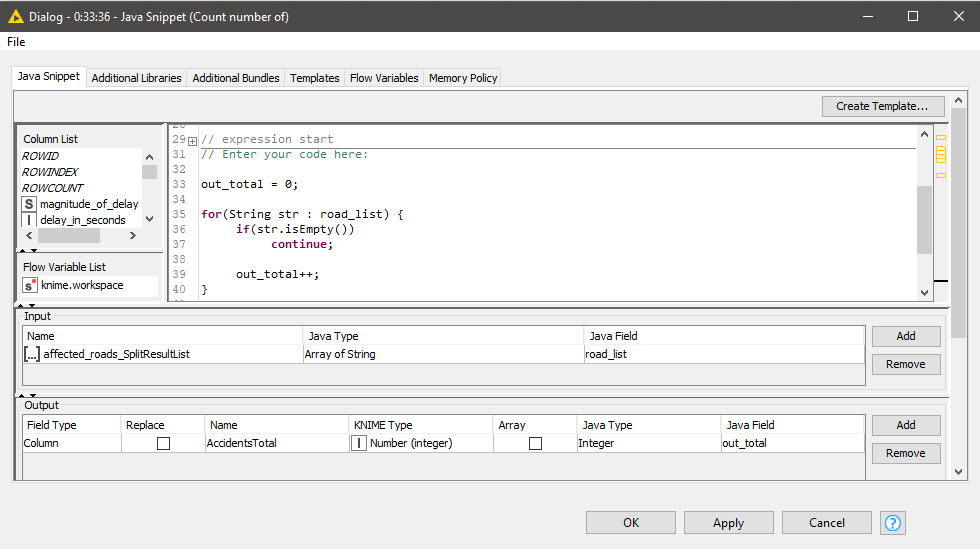
\includegraphics[scale=0.3
                ]{Figures/wf_braga_roadCount.png}
                \caption{Visão geral do workflow gerado para trabalhar o dataset.}
                \label{fig:"um"}
            \end{figure} 
            De seguida convertemos o valor de alguns campos relativos a "magnitude\_of\_delay". Optámos por converter as classes deste campo que tinham uma baixa frequência para a classe "MODERATE".
            
        \item \textbf{Hyper Parameter Tuning} \\
            Para melhorarmos a precisão do modelo gerado optamos por fazer um "tuning" dos parâmetros utilizados. Para o fazer utilizamos loops, testando diferentes combinações entre os critérios de divisão de Random Forests e múltiplos valores para o número de modelos e profundidade da árvore. Uma vez terminados estes loops passamos os valores obtidos como "ideais" para variável de flow e treinamos um modelo com estas definições, já no próximo ponto. Pode ser vista uma representação desta parte do processo mais á frente, mais concretamente na secção "Descrição do modelo gerado".
        
        \item \textbf{Previsões} \\
            Uma vez optimizados os parâmetros do modelo procedemos ao treino do mesmo, para o efeito utilizando um \textit{Random Forest Learner}. Com o modelo gerado prevemos o nível de acidentes para cada um dos registos presentes no \textit{dataset} de teste. Os resultados desta previsão são então exportados, de acordo com as regras estabelecidas para a competição na plataforma \textit{Kaggle}.
    \end{enumerate}
    
    \subsubsection{Descrição do modelo gerado}
        \begin{enumerate}
            \item \textbf{Tuning}    
                \begin{figure}[H]
                    \centering
                    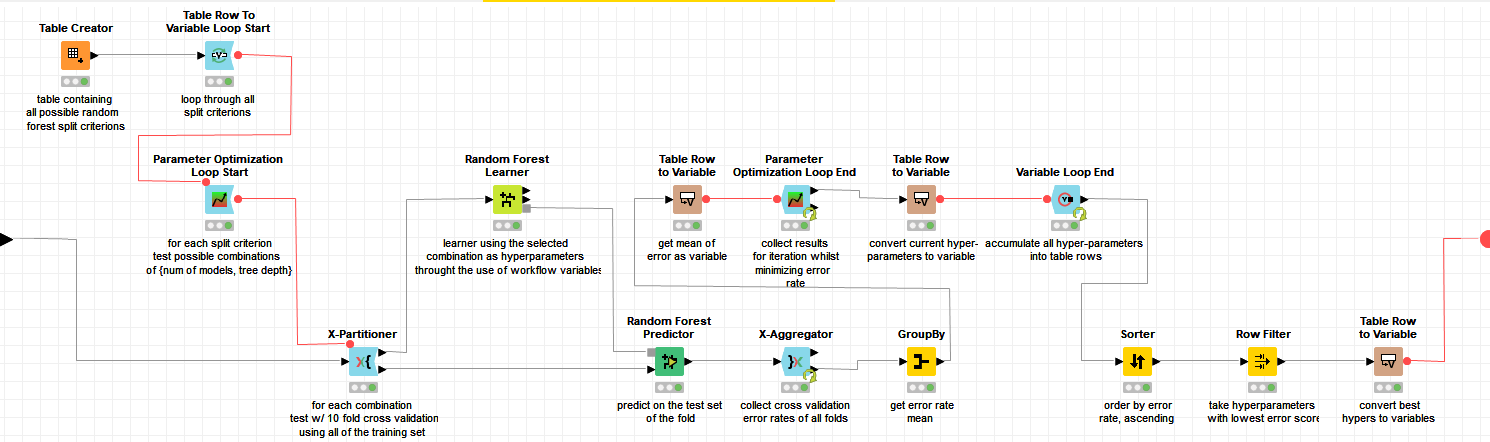
\includegraphics[scale=0.30
                    ]{Figures/wf_braga_hyper.png}
                    \caption{Metanodo utilizado para optimização do hiper-parâmetros.}
                    \label{fig:"um"}
                \end{figure} 
                
            \item \textbf{Características do treino}
                Após terminado o loop de optimização temos então os valores óptimos para a nossa \textit{Decision Tree}. No caso em concreto os parametros "ideais" foram os seguintes:
                \begin{itemize}
                    \item Número de modelos: 700
                    \item Profundidade da árvore: 25
                    \item Split Criterions: Information Gain
                \end{itemize}
                \begin{figure}[H]
                    \centering
                    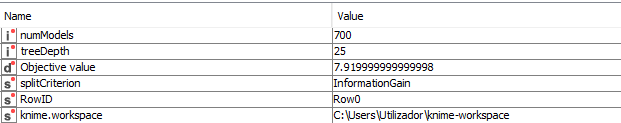
\includegraphics[scale=0.30
                    ]{Figures/wf_braga_hyperdata.png}
                    \caption{Settings utilizados para treino do modelo.}
                    \label{fig:"um"}
                \end{figure} 
        \end{enumerate}